\documentclass{article}

% \usepackage{draftwatermark}
% \SetWatermarkText{Draft}
% \SetWatermarkScale{5}
% \SetWatermarkLightness {0.9} 
% \SetWatermarkColor[rgb]{0.7,0,0}


\usepackage{geometry}                		% See geometry.pdf to learn the layout options. There are lots.
\geometry{letterpaper}                   		% ... or a4paper or a5paper or ... 
%\geometry{landscape}                		% Activate for for rotated page geometryhttps://www.washingtonpost.com/world/europe/amid-impeachment-probe-gordon-sondland-is-overseeing-a-renovation-of-his-residence-that-has-cost-1-million-in-taxpayer-money/2019/10/16/d0eece92-ef86-11e9-bb7e-d2026ee0c199_story.html?tid=sm_tw
%\usepackage[parfill]{parskip}    		% Activate to begin paragraphs with an empty line rather than an indent
\usepackage{graphicx}				% Use pdf, png, jpg, or eps� with pdflatex; use eps in DVI mode
								% TeX will automatically convert eps --> pdf in pdflat						\label{thm:integral_domain}

								% TeX will automatically convert eps --> pdf in pdflatex		
\usepackage{amssymb}
\usepackage{amsmath}
\usepackage{amsthm}
\usepackage{mathrsfs}
\usepackage[hyphens,spaces,obeyspaces]{url}
\usepackage{url}
\usepackage{hyperref}
\usepackage{subcaption}
\usepackage{authblk}
\usepackage{mathtools}
\usepackage{graphicx}
\usepackage[export]{adjustbox}
\usepackage{fixltx2e}
\usepackage{hyperref}
\usepackage{alltt}
\usepackage{color}
\usepackage[utf8]{inputenc}
\usepackage[english]{babel}
\usepackage{float}
\usepackage{bigints}
\usepackage{braket}
\usepackage{siunitx}
\usepackage{mathtools}


\usepackage{tikz}
\usepackage{verbatim}
\usetikzlibrary{plotmarks}
\usepackage{pgfplots}
\usepackage{amsmath}
 \usepackage{relsize}
 
 \usepackage[hyphenbreaks]{breakurl}
 
 \newtheorem{thm}{Theorem}[section]
% \newtheorem{defn}[thm]{Definition}
\theoremstyle{definition}
\newtheorem{definition}{Definition}[section]
\newtheorem{proposition}{Proposition}[section]
\newtheorem{lemma}{Lemma}[section]
\newtheorem{example}{Example}[section]

\newcommand{\argmax}{\operatornamewithlimits{argmax}}
\newcommand{\argmin}{\operatornamewithlimits{argmin}}




\title{A Few Notes On The Dirac Delta Function}
\author{David Meyer \\ dmm@\{1-4-5.net,uoregon.edu,...\}}

\date{Last update: \today}							% Activate to display a given date or no date

\begin{document}
\maketitle

\section{Introduction}
These notes began life as some thoughts on the Dirac Delta Function and evolved into notes on several related topics including  Laplace Transforms. The 
Dirac Delta function has all kinds of crazy and interesting properties. More TBD.

\section{The Dirac Delta Function}
The Dirac Delta Function is defined as shown in Figure \ref{fig:delta}. In the limit ($\mathlarger{\epsilon} \to 0$) the
 Dirac Delta function is written $\delta_a(t)$ or sometimes $\delta(t - a)$. As we will see in a moment, the $\delta_{a,\epsilon}(t)$ form of the delta function
 is useful when we want to use the Mean Value Theorem for Integrals \cite{wiki:meam_value_theorem_for_integrals} to evaluate integrals involving the delta function.
 
\bigskip

\begin{figure}[H]
  \centering
  \begin{tikzpicture}[scale=2.0]
     \draw [<->] (0,3) -- (0,0) -- (4,0);                                                                      % draw axes
     \draw (3,2) node[rectangle] {                                                                           % draw function to the right
         $\delta_{a,\epsilon}(t) =  
           \begin{cases} 
             \frac{1}{\mathlarger {\epsilon}} & a \leq t \leq a + \epsilon \\
             0                                               & \text{otherwise}
           \end{cases}$
       }; 
     \draw [dashed] (1,0) node[below] {$a$}                 -- (1,1); 
     \draw [dashed] (2,0) node[below] {$a + \epsilon$} -- (2,1);
     \coordinate (y) at (0,1); \fill [black] (y) circle (1pt);                                           % draw a dot on the y axis (I'd like to make it smaller but I don't see how)
     \draw (0,1) node[left] {$\frac{1}{\mathlarger{\epsilon}}$};
     \draw [thick,red] (0,0) -- (1,0);
     \draw [thick,red] (2,0) -- (4,0);
     \draw [thick,red] (1,1) -- (2,1);
     \draw [dashed]   (0,1) -- (1,1);
     \draw (4,0) node [label=right:{$t$}] {};
     \draw (0,3) node [label=above:{$\delta_{a,\epsilon}(t)$}] {};
  \end{tikzpicture}
  \caption{The Dirac Delta Function $\delta_{a,\epsilon}(t)$}
  \label{fig:delta}
\end{figure}

\bigskip
\noindent
So $\delta_{a,\epsilon}(t)$ is defined to be

\begin{equation*}
\delta_{a,\epsilon}(t) =  
 \begin{cases} 
      \frac{1}{\mathlarger {\epsilon}} & a \leq t \leq a + \epsilon \\
      0                                               & \text{otherwise}
   \end{cases}
\label{eqn:delta}
\end{equation*}

\noindent
\bigskip
and has the constraint that


\begin{equation*}
  \int_{0}^{\infty} \delta_{a,\epsilon}(t) =  1
\end{equation*}

\bigskip
\bigskip
\noindent
\bigskip
That is, $\delta_{a,\epsilon}(t)$ is in some sense a probability density.

\bigskip
\noindent
In the limit the Dirac Delta Function looks like

\begin{equation*}
\lim_{\epsilon \to 0} \delta_{a,\epsilon}(t) =
\delta_{a}(t) =  
 \begin{cases} 
     \infty & t = a\\
      0     & t \neq a
   \end{cases}
\end{equation*}

\bigskip
\noindent
or sometimes

\begin{equation*}
\delta (t - a) =  
  \begin{cases} 
     0 & t \neq a\\
      \infty     & t = a
  \end{cases}
\end{equation*}

\bigskip
\noindent
$\delta_a(t)$ also has the constraint that 


\begin{equation*}
  \int_{0}^{\infty} \delta_{a}(t) =  1
\end{equation*}

\bigskip
\noindent
and so is also a probability density. $\delta_a(t)$  is shown in Figure \ref{fig:delta_limit}.

\begin{figure}[H]
  \centering
  \begin{tikzpicture}[scale=2.0]
     \draw [<->] (0,2) -- (0,0) -- (4,0);                                                                      % draw axes
     \draw (3,1) node[rectangle] {                                                                           % draw function to the right
         $\delta_{a}(t) =  
           \begin{cases} 
              \infty & t = a  \\
               0      & \text{otherwise}
           \end{cases}$
       }; 
     \draw (1,0) node[below] {$a$};
     \draw [dashed,red] (1,0) -- (1,2);
     \draw (4,0) node [label=right:{$t$}] {};
     \draw (0,2) node [label=above:{$\delta_{a}(t)$}] {};
     \draw [thick,red] (0,0) -- (1,0);
     \draw [thick,red] (1,0) -- (4,0);
  \end{tikzpicture}
  \caption{The Dirac Delta Function $\delta_{a}(t)$}
  \label{fig:delta_limit}
\end{figure}


\subsection{Integrals Involving $\delta_{a,\epsilon}(t)$}
$\delta_{a,\epsilon}(t)$ has all kinds of interesting properties. One of them involves the integral of the product $\delta_{a,\epsilon}(t)$ with some function $g(t)$.  
Here we would like to evaluate integrals of the form

\bigskip
\begin{equation}
  \int_{0}^{\infty} \delta_{a,\epsilon}(t) g(t) dt
  \label{eqn:delta_integral}
\end{equation}

\bigskip
\noindent
where $g(t)$ is continuous on the interval $[a, a+\epsilon]$. 
 
\bigskip
\noindent
The Mean Value Theorem for Integrals  \cite{wiki:meam_value_theorem_for_integrals}  tells us that

\begin{equation}
  \int_{a}^{b} g(t) dt = (b -a) g(c)
  \label{eqn:mvti}
\end{equation}

\bigskip
\noindent
where the point $c$ lies in the interval $[a, a+\epsilon]$. Now, since we know that $\delta_{a,\epsilon}(t)$ is zero everywhere except on the interval
$[a, a+\epsilon]$ we can rewrite the improper integral in Equation \ref{eqn:delta_integral} as the proper integral

\begin{equation*}
  \int_{a}^{a + \epsilon} \delta_{a,\epsilon}(t) g(t) dt
\end{equation*}

\bigskip
\noindent
Here we can notice that $ \delta_{a,\epsilon}(t) = \frac{1}{\mathlarger{\epsilon}}$ on the interval $[a, a+\epsilon]$ so we can rewrite our integral as 

\bigskip
\begin{equation*}
  \int_{a}^{a + \epsilon} \frac{1}{\mathlarger{\epsilon}} g(t) dt =  \frac{1}{\mathlarger{\epsilon}} \int_{a}^{a + \epsilon} g(t) dt
\end{equation*}

\bigskip
\noindent
Now we can use Equation \ref{eqn:mvti}, the Mean Value Theorem for Integrals\footnote{This is where the $\delta_{a,\epsilon}(t)$ form of the delta function comes in handy.},
by setting $b = a + \epsilon$ and $a = a$ so that $b - a = \epsilon$. Then 

\bigskip
\begin{equation*}
 \frac{1}{\mathlarger{\epsilon}} \int_{a}^{a + \epsilon} g(t) dt =  \frac{1}{\mathlarger{\epsilon}} \underbrace{ \Big [(a + \epsilon) - a \Big]}_{b -a} g(c) = \frac{1}{\mathlarger{\epsilon}} \epsilon g(c) = g(c)
\end{equation*}

\bigskip
\noindent
where $c \in [a, a + \epsilon]$. 

% \newpage
\bigskip
\noindent
Finally, if we look at what happens to $c$ as $\epsilon \to 0$ we see that $\lim\limits_{\epsilon \to 0} c = a$ (sorry about the notation abuse)
so that 

\begin{equation}
  \int_{0}^{\infty} \delta_{a}(t) g(t) dt = g(a)
  \label{eqn:g(a)}
\end{equation}

\bigskip
\noindent
Essentially $\delta_{a}(t)$ pulls out the value of $g$ at $a$, that is, $g(a)$.

\bigskip
\noindent
Another way to get this result \cite{youtube:suskind2008.4} is to notice that the integrand of 

\bigskip
\begin{equation*}
  \int_{0}^{\infty} \delta (t-a) g(t) dt
\end{equation*}

\bigskip
\noindent
is zero everywhere except where $t = a$, so we can rewrite our integral as
 $\int_{0}^{\infty} \delta (t-a) g(a) dt = g(a) \int_{0}^{\infty} \delta (t-a) dt$ (since $g(a)$ doesn't depend on $t$). 
 Then since by definition $ \int_{0}^{\infty} \delta (t-a) dt = 1$ we get

\bigskip
\begin{equation*}
  \int_{0}^{\infty} \delta (t-a) g(t) dt = g(a)
\end{equation*}

\bigskip
\section{The Laplace Transform}
We start by defining the integral transform of some function $f(t)$.

\bigskip
\begin{definition} 
{\bf Integral Transform}
\end{definition}

\noindent
If a function $f(t)$ is defined on $[0,\infty)$ then we can define an integral transform to be the improper integral


\begin{equation*}
F(s) = \int_0^\infty K(s,t) f(t) dt
\end{equation*}

\bigskip
\noindent
If the improper integral converges then we say that $F(s)$ is the integral transform of $f(t)$. The function $K(s,t)$ is called the \emph{kernel}
of the transform. When $K(s,t) = e^{-st}$ the transform is called the {\bf Laplace Transform}.

\bigskip
\begin{definition} 
{\bf Laplace Transform}
\label{def:laplace_transform}
\end{definition}

\bigskip
\noindent
The Laplace Transform of a function $f(t)$ is defined to be


\bigskip
\begin{equation*}
\mathcal{L}\{f(t)\} = F(s) = \int_0^\infty f(t) e^{-st} dt
\end{equation*}

\bigskip
\noindent
and is useful when solving ordinary differential equations (ODEs). Interestingly, the Laplace Transform of the Dirac Delta Function turns out to be

\bigskip
\begin{equation*}
\begin{array}{lllll}
\mathcal{L}\{\delta_a(t)\} 
&=& \int_0^\infty  \delta_a(t) e^{-st} dt    &\quad  \mathrel{\#} \text{definition of the Laplace Transform}  \\  
[4pt]                                                        % get a bit of space
&=& \int_0^\infty \delta_a(t) g(t)  dt        &\quad  \mathrel{\#} \text{set $g(t) = e^{-st}$}                            \\
[4pt]                                                        % get a bit of space
&=& g(a)                                                &\quad  \mathrel{\#} \text{by Equation \ref{eqn:g(a)}}                 \\
[4pt]                                                        % get a bit of space
&=& e^{-sa}                                            &\quad  \mathrel{\#} \text{since $g(t) = e^{-st}$}
\end{array}
\end{equation*}

\subsection{The Linearity Property Of The Laplace Transform}
\bigskip
\noindent
$\mathcal{L}$ is a linear operator, in other words: $\mathcal{L}\{af (t) + bg(t)\} = a\mathcal{L}\{f(t)\} + b\mathcal{L}\{g(t)\}$. Why? Consider:


\begin{equation*}
\begin{array}{lllll}
\mathcal{L}\{af (t) + bg(t)\} 
&=& \int_0^\infty e^{-st} \big [\mathcal{L}\{af (t) + bg(t)\} \big] dt          & \mathrel{\#} \text{definition of the Laplace Transform (Definition \ref{def:laplace_transform})}  \\  
[10pt]                                                                                                    % get a bit of space
&=& a \int_0^\infty e^{-st}  f(t) dt + b \int_0^\infty e^{-st}  g(t) dt           & \mathrel{\#} \text{by the linearity of improper integrals \cite{lewis2014}}                                    \\
[10pt]                                                                                                    % get a bit of space
&=& a \mathcal{L}\{f(t)\}  + b \mathcal{L}\{g(t)\}                                   & \mathrel{\#} \text{definition of the Laplace Transform} 
\end{array}
\end{equation*}

\subsection{So Does Every Function Have A Laplace Transform?}
The answer is no (consider a function like $f(t) = t^{-1}$). There are two properties that $f(t)$ must have in order to have a Laplace Transform. First, $f(t)$ must
be of "exponential order". So what does that mean?

\bigskip
\begin{definition} 
{\bf Exponential Order}
\label{def:exponential_order}
\end{definition}
\noindent
A function $f$ is said to be of {\bf exponential order $c$} if there exist constants $c, M > 0, \text{ and } T > 0$ such that $|f(t)| \leq Me^{ct}$ for all $t > T$.

\bigskip
\noindent
Basically this is saying that in order for $f(t)$ to have a Laplace Transform then in a race between $|f(t)|$ and $e^{ct}$ as $t \to \infty$ $e^{ct}$ must
approach its limit first. Said another way:  

\bigskip
\begin{equation*}
\lim\limits_{t \to \infty} \frac{f(t)}{e^{ct}} = 0
\end{equation*}

\bigskip
\noindent
This is shown in Figure \ref{fig:exponential_order}.

\bigskip
\begin{figure}[H]
\center{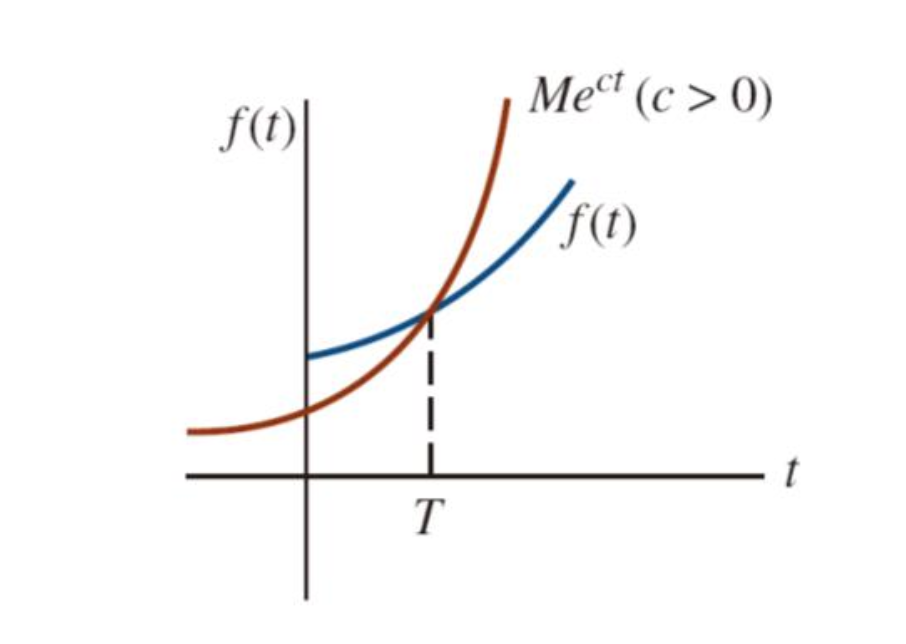
\includegraphics[scale=0.50,frame] {images/exponential_order.png}}
\caption{$f(t)$ is of exponential order with constants $c, M$ and $T$}
\label{fig:exponential_order}
\end{figure}

\bigskip
\noindent
Next we need the following theorem:

% \newpage
\bigskip
\begin{thm} 
{\bf Existence Theorem:} 
\normalfont If $f$ is s piecewise continuous on the interval $[0,\infty)$ and is of exponential order $c$ then 
$F (s) = \mathcal{L}\{f (t)\} \text{ is defined for all $s > c$}.$
\end{thm}

\bigskip
\noindent
Ok, but why? Consider

\begin{equation*}
\begin{array}{lllll}
\mathcal{L}\{f(t)\}
&=& F(s)                                                                            &\quad  \mathrel{\#} \text{definition of the Laplace Transform (Definition \ref{def:laplace_transform})}                                                             \\  
[10pt]                                                                                 % get a bit of space
&=& \int_0^\infty e^{-st} f(t) dt                                            &\quad  \mathrel{\#} \text{definition of the Laplace Transform (Definition \ref{def:laplace_transform})}                                                              \\  
[10pt]                                                                                 % get a bit of space
&\leq& \int_0^\infty e^{-st}  Me^{ct}dt                                &\quad  \mathrel{\#} \text{$f$ is of exponential order $c$ (Definition \ref{def:exponential_order})}                                                                     \\  
[10pt]                                                                                 % get a bit of space               
&=& M  \int_0^\infty e^{-st} e^{ct} dt                                  &\quad  \mathrel{\#} \text{$M$ doesn't depend on $t$}                                                                                                                                       \\   
[10pt]                                                                                 % get a bit of space
&=& M  \int_0^\infty  e^{(c-s)t}  dt                                      &\quad  \mathrel{\#} \text{collect powers of $e$}                                                                                                                                                \\      
[10pt]                                                                                 % get a bit of space
&=&  M \int_0^\infty e^u dt                                                &\quad  \mathrel{\#} \text{use a $u$ substitution with $u = (c-s)t$}                                                                                                                     \\     
[10pt]                                                                                 % get a bit of space
&=&  M \int_0^\infty e^u \frac{du}{c-s}                              &\quad  \mathrel{\#} \text{$du = (c-s) dt \: \Rightarrow \: dt = \dfrac{du}{c-s}$}                                                                                                    \\     
[10pt]                                                                                % get a bit of space
&=& \Big [ \frac{M}{c-s} \Big ] \int_0^\infty e^u du            &\quad  \mathrel{\#} \text{neither $c$ nor $s$ depend on $t$}                                                                                                                             \\     
[10pt]                                                                                % get a bit of space
&=& \Big [ \frac{M}{c-s} \Big ] e^u \Big |_0^\infty              &\quad  \mathrel{\#} \int_0^\infty e^u du = e^u +C                                                                                                                                               \\     
[10pt]                                                                                % get a bit of space
&=& \Big [ \frac{M}{c-s} \Big ]  e^{(c-s)t} \Big |_0^\infty     &\quad  \mathrel{\#} u = (c-s)t                                                                                                                                                                              \\
[10pt]                                                                                % get a bit of space     
&=& \lim\limits_{d \to \infty}\Big [\frac{M}{c-s} e^{(c-s)d} \Big ] - \frac{M}{c - s}e^{(c-s)0}  &\quad \mathrel{\#} \text{evaluate at the limits}                                                                                                   \\
[10pt]                                                                                % get a bit of space
&=& \lim\limits_{d \to \infty}\Big [\frac{M}{c-s} e^{(c-s)d} \Big ] - \frac{M}{c - s}                 &\quad  \mathrel{\#} e^{(c-s)0} = 1 \text{ and } \frac{M}{c-s} \cdot 1 = \frac{M}{c-s}                                             \\
[10pt]                                                                                % get a bit of space
&=& 0 - \frac{M} {\mathlarger{c-s}}                                   &\quad  \mathrel{\#} \text{we assumed that $s > c$ so $c -s < 0 \Rightarrow  \lim\limits_{d \to \infty}\Big [\frac{M}{c-s} e^{(c-s)d} \Big ] = 0$}   \\    
[10pt]                                                                                % get a bit of space
&=& \frac{M}{\mathlarger{s-c}}                                         &\quad  \mathrel{\#} \text{simplify} 
\end{array}
\end{equation*}

\bigskip
\noindent
All of this implies that functions $f(t)$ that do not satisfy the Existence Theorem do not have Laplace Transforms since $\mathcal{L}\{f(t)\}$ doesn't converge.


% \newpage
\bigskip
\section*{Acknowledgements}

\newpage
\bibliographystyle{plain}
\bibliography{/Users/dmm/papers/bib/qc}
\end{document}